% !TeX encoding = UTF-8
% !TeX spellcheck = en_US
\documentclass[twocolumn,a4paper,9pt]{article}

\usepackage[utf8x]{inputenc}
%\usepackage[french]{babel}

\frenchspacing{}
\usepackage[cm]{fullpage}
\usepackage[output-decimal-marker={,}]{siunitx}
\usepackage{enumerate}
\usepackage{hyperref}

\usepackage{multirow,hhline,colortbl,threeparttable,graphicx,xcolor}

\usepackage{lmodern}
\usepackage{erewhon} %, uppercase=upright
\usepackage[protrusion=true,expansion]{microtype}

\title{A \LaTeX{} Tool to Develop Content-Rich Moodle Quizzes}
\author{C. \textsc{Barès}, F. \textsc{Goutailler}, and M. 
\textsc{Guerquin-Kern}\footnote{principal investigator. Contact: 
\href{mailto:guerquin@ensea.fr}{guerquin@ensea.fr}}}
\date{2019}

\begin{document}

\maketitle
\tableofcontents

\section{Context}

This document is a proposal for the project call ``\emph{création de cours en 
ligne à contenu enrichi}'' for the academic year 2018-2019.

\subsection{Moodle Quizzes at ENSEA}

ENSEA currently supports the creation of Moodle quizzes. For each teaching 
module, 67 working hours (16 HETD) are allocated to the mission \emph{création 
d’outil numérique en lien avec un module d’enseignement}.

\subsection{Pedagogical Interests}

Assessment for Learning (AfL) is a way to encourage students to be more active 
in their learning. Its five big principles were identified by the UK Assessment 
Reform Group in 1999:
\begin{enumerate}
	\item provision of effective feedback to students,
	\item active involvement of students in their own learning,
	\item adjusting teaching to take account of the results of assessment,
	\item recognition of the profound influence assessment has on the 
	motivation and self-esteem of pupils, both of which are critical influences 
	on learning, and
	\item need for students to be able to assess themselves and understand how 
	to improve.
\end{enumerate}

Moodle quizzes may very well serve in the scope of AfL.

First, Moodle quizzes are quite versatile, with a wide variety of questions. 
Third-party plugins offer special question types, but by default, the main 
question types that Moodle supports are:
\begin{itemize}
\item \emph{Multiple choice} Options are: single or multiple expected 
answers, shuffled or unshuffled.
\item \emph{Numerical value} Tolerance can be specified
\item \emph{Short answer} Options are: case sensitive or case insensitive.
\item \emph{Matching} Options are: shuffled or unshuffled.
\item \emph{Essay} Different answer formats are available: text, html, file 
import\dots
\item \emph{Cloze} is a type of question that embeds one or several multiple 
choice, short answer, or numerical questions.
\end{itemize}

Second, Moodle's quizz questions can offer different levels of feedbacks 
to the student:
\begin{itemize}
	\item General feedback, displayed whatever the student's answer is;
	\item Overall feedbacks, that can be tuned for correct, partially correct, 
	and incorrect responses;
	\item Answer-specific feedbacks, that depend on the specific answer the 
	student gives.
\end{itemize}
Moodle quizzes can be used in teaching to support learning activities by 
targeting common mistakes, errors, and misconceptions. In this case, we believe 
that answer-specific feedback is a very valuable tool.

Third, if the other teaching activities are integrated in Moodle, Moodle 
quizzes taken in the scope of AfL can be made mandatory, possibly with a 
minimum grade. The achievement of the assessment can be made to trigger 
unveiling following course contents or activities. The teacher can monitor 
students advancement and results.

Finally, Moodle's automatic assessment of quizzes offers interesting 
perspectives for giving regular, detailed and tailored feedback to large 
cohorts of students.

\subsection{Frustration of Editing Quizzes on Moodle}

Probably most of the teachers that have tried to create quizzes on Moodle have 
experienced frustration. This frustration might prevent or limit teachers in 
the processes of creating or editing such quizzes with the quality and quantity 
that would be required by AfL. In the \LaTeX{} \texttt{moodle} package 
documentation, Anders Hendrickson found the words to describe the different 
shortcomings that teachers encounter:
\begin{itemize}
\item \emph{the agonizing slowness of switching between mouse and keyboard to 
navigate a web form with its myriad dropdown boxes, radio buttons, compounded 
with a perceptible time lag as one’s Moodle server responds to requests, can 
produce a very frustrating experience}
\item \emph{editing is entirely impossible without network access}
\item \emph{once the quiz is written, there is no easy way to view and 
proofread all the information of which it is made. Each question is edited on a 
separate webpage, which is so full of options that it cannot be viewed on a 
single screen. An instructor has to spend much time checking over the newly 
created quiz in order to be confident there are no errors.}
\item \emph{frustration of managing graphics. If a question requires
an image, the image must first be produced as a standalone file (e.g., in JPG 
or PNG format), uploaded to Moodle, and then chosen in a web-based HTML editor. 
Great is the vexation of the instructor who decided to alter a question, as 
there are more and more possibilities of error whenever multiple files must be 
kept synchronized.}
\end{itemize}

To this list, we add our frustration of not being able to:
\begin{itemize}
	\item easily make small variations of existing questions
	\item reuse our own teaching material: images, \LaTeX{} code and macros.
\end{itemize}

\subsection{Tools Made to Alleviate This Frustration}

Fortunately, Moodle offers several ways to import or export a question bank. 
Among these is a very comprehensive XML format.

Based on this feature, some initiatives have emerged to offer third-party tools 
capable of editing questions in a way that is more convenient to the teacher. 
Because they are not in use at ENSEA, we do not discuss here the different 
Virtual Learning Environments that have their own format that can be imported 
by moodle: Blackboard, Examview, Hot Potatoes, Learnwise, WebCT.

First, VLE Tools~\cite{vletools} is a free online service, available after 
registration. The description of the questions is text-based. 
Images cannot be imported. There is also a paid service for the conversion of 
questions from raw material.% \LaTeX{} code?

Second, the tool Moodle2Word~\cite{moodle2word} is made for 
the users of Word of the Microsoft Office suite. It allows to export existing 
Moodle question banks to the Word format for archive and editing purposes, and 
importing back to Moodle. Images and \LaTeX{} code are supported. It requires 
the installation of a Moodle plugin. Figure~\ref{fig:moodle2word} shows a 
question edited with this tool.

\begin{figure}[tbp]
\centering
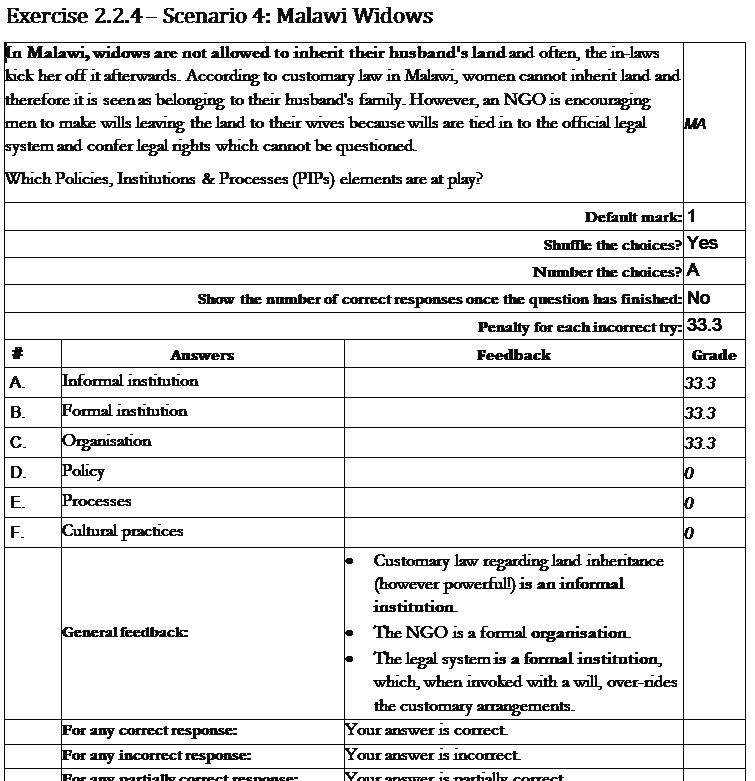
\includegraphics[width=.5\textwidth]{moodle2word}
\caption{Example of a question edited with moodle2word, taken from ``The 
Marriage of Moodle (and Word)'' by Eoin Campbell}
\label{fig:moodle2word}
\end{figure}

Finally, the \texttt{moodle} \LaTeX\ package~\cite{latex2moodle} is the 
Moodle2Word counterpart for \LaTeX{} users. It is capable of dealing with 
images and, of course, \LaTeX{} code. The conversion works only from \LaTeX{} 
to XML. Figure~\ref{fig:latex2moodle} shows questions edited with this tool.

\begin{figure*}[tbp]
\centering
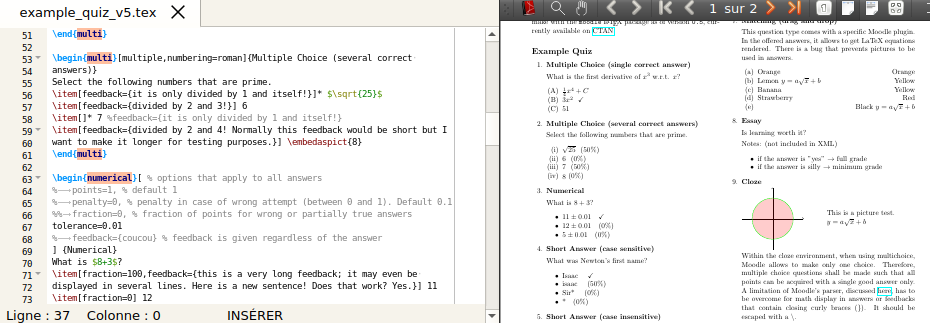
\includegraphics[width=\textwidth]{latex2moodle}
\caption{Example of questions edited with the \LaTeX\ package \texttt{moodle}}
\label{fig:latex2moodle}
\end{figure*}

\section{Proposed Working Directions}

With this project, we propose to improve the existing \LaTeX{} package named 
\texttt{moodle}, currently distributed with version number \texttt{0.5}.
We tried to reach the author and maintainer of this package with no success. 
This appear now to be an unmaintained piece of work, mainly developed and 
tested during one academic semester in 2016.

We identified several fields that would require improvement.

\subsection{Bug Fixing}

Table~\ref{tab:2} lists the bugs and limitations that we found are impairing 
content enrichment with the current package (version \texttt{0.5}).

\begin{table*}[tbp]
\centering
\def\OKcell{\cellcolor{green}}
\def\KOcell{\cellcolor{red}}
\def\DNAcell{\cellcolor{black!20}} % "Does not apply"
\def\Warncell{\cellcolor{orange}} % Warning
\def\MyLine{\hhline{~-|>{\arrayrulecolor{green}}->{\arrayrulecolor{black}}--|>{\arrayrulecolor{green}}->{\arrayrulecolor{black}}--|}
}
\begin{threeparttable}[b]
\caption{Content enrichment support after XML import in Moodle 
\texttt{v3.1}, depending on the question type. Color convention: green for 
\colorbox{green}{full support}, orange for \colorbox{orange}{problems limiting 
the support}, red for \colorbox{red}{show-stopping problems}, and gray for 
\colorbox{black!20}{support limitations intrinsic to the question type} defined 
by Moodle.}
\label{tab:2}
\begin{tabular}{rl|ccc|ccc}
\multicolumn{2}{c|}{}& \multicolumn{3}{c|}{\LaTeX{} equation 
rendering} & \multicolumn{3}{c}{Picture inclusion}\\
\multicolumn{2}{c|}{Question type}& Question & Answer & Feedback & 
Question & Answer & Feedback\\\hhline{*{8}{:=}:}

&\href{https://docs.moodle.org/31/en/Multiple_Choice_question_type} 
{Multichoice} \emph{bug\tnote{1}} & \OKcell & \OKcell & \KOcell 
bug\tnote{2} & \Warncell bug\tnote{12} & \Warncell bug\tnote{12} & \KOcell 
bug\tnote{2}, bug\tnote{12}\\\hhline{*{8}{-}}

& \href{https://docs.moodle.org/31/en/Numerical_question_type}{Numerical}
& \OKcell & \DNAcell Text only\tnote{3} & \KOcell bug\tnote{2} & 
\OKcell bug\tnote{12} & \DNAcell Text only\tnote{3} & \KOcell 
bug\tnote{2}, bug\tnote{12}\\\hhline{*{8}{-}}

& \href{https://docs.moodle.org/31/en/Short-Answer_question_type}{Short Answer} 
& \OKcell & \DNAcell Text only\tnote{3} & \KOcell bug\tnote{2}& \OKcell 
bug\tnote{12} & \DNAcell Text only\tnote{3} & \KOcell bug\tnote{2}, 
bug\tnote{12}\\\hhline{*{8}{-}}

& Matching 
(\href{https://docs.moodle.org/31/en/Matching_question_type}{standard})
& \OKcell & \DNAcell Text only\tnote{4} & \DNAcell Irrelevant\tnote{5} & 
\OKcell & \DNAcell Text only\tnote{4} & \DNAcell Irrelevant\tnote{5} 
\\\hhline{*{8}{-}}

&Matching 
(\href{https://docs.moodle.org/31/en/Drag_and_drop_matching_question_type}{drag-and-drop})
& \OKcell & \DNAcell bug\tnote{13} & \DNAcell Irrelevant\tnote{5} & 
\OKcell bug\tnote{12}& \DNAcell bug\tnote{12}, bug\tnote{13}& \DNAcell 
Irrelevant\tnote{5} \\\hhline{*{8}{-}}

&\href{https://docs.moodle.org/31/en/Essay_question_type}{Essay} 
\emph{bug\tnote{6}, note\tnote{11}} & \OKcell & \Warncell 
note\tnote{7}, bug\tnote{8} & \OKcell note\tnote{7} & \Warncell bug\tnote{12} & 
\Warncell note\tnote{7}, bug\tnote{8} & \Warncell note\tnote{7}, 
bug\tnote{12}\\\hhline{*{8}{-}}

\multirow{5}{*}{ 
\href{https://docs.moodle.org/31/en/Embedded_Answers_(Cloze)_question_type}
{Cloze}}

&Numerical & \OKcell & \DNAcell Text only\tnote{3} & \KOcell 
bug\tnote{2}, bug\tnote{9} & \OKcell & \DNAcell Text only\tnote{3} & \KOcell 
bug\tnote{2}\\\MyLine

&Short Answer & \OKcell & \DNAcell Text only\tnote{3} & \KOcell 
bug\tnote{2}, bug\tnote{9}, note\tnote{10} & \OKcell & \DNAcell Text 
only\tnote{3} & \KOcell bug\tnote{2}, note\tnote{10}\\\MyLine

&Multi (dropdown) & \OKcell & \DNAcell Text only\tnote{4} & \KOcell 
bug\tnote{2}, bug\tnote{9}, note\tnote{10} & \OKcell & \DNAcell 
Text only\tnote{4} & \KOcell bug\tnote{2}, note\tnote{10} \\\MyLine

&Multi (horizontal)& \OKcell & \Warncell bug\tnote{9} & \KOcell 
bug\tnote{2}, bug\tnote{9} & \OKcell & \OKcell & \KOcell bug\tnote{2}\\\MyLine

&Multi (vertical)& \OKcell & \Warncell bug\tnote{9} & \KOcell 
bug\tnote{2}, bug\tnote{9} & \OKcell & \OKcell & \KOcell 
bug\tnote{2}\\\hline
\end{tabular}
\begin{tablenotes}
\item[1] Numbering with option ``ABC" is not recognized by Moodle 
after XML import.
\item[2] Any $\backslash$ symbol here breaks \LaTeX{} compilation. 
For instance, this prevents the use of \verb|\includegraphics|, 
\verb|\begin| and \verb|\sqrt|.
\item[3] Moodle prompts the student for an answer and then compares 
it to the solutions provided. This is text-only.
\item[4] Moodle uses a dropdown list to let one choose among the 
possible answers. This forbids either picture inclusion and \LaTeX{} 
rendering.
\item[5] Not supported by Moodle (in this context, answer-specific 
feedback represents lots of possible combinations).
\item[6] The keyval ``response template", as documented, is broken. 
Works if replaced with ``template".
\item[7] For this question type and in the context of XML 
generation, the Answer column represents the ``template" while the Feedback 
column represents the ``notes for the grader". Obviously, the grading process 
is not automatic and there is no answer-specific feedback.
\item[8] Picture and \LaTeX{} rendering could be done, but only 
after submission and only if the keyval "response format" was set to 
``html". 
Unfortunately, the \texttt{<p>...</p>} tags introduced, whatever 
the response format is, prevent rendering.
\item[9] In the generated XML, the symbol $\}$ is not escaped with 
a backslash as required by the Moodle cloze parser. The XML import will fail 
when the field contains \LaTeX{} code like \verb|\sqrt{...}| and 
\verb|\frac{...}{...}|.
\item[10] Moodle only reveals the feedback when hovering the 
checkmark or X mark with the mouse.
\item[11] When generating an Essay, a note is added to the PDF 
saying ``Notes: (not included in XML)". Instead, the notes are included in the 
XML and available to the grader after import on Moodle.
\item[12] In the XML, the pictures included in the question field 
and answer or feedback fields are mixed.
\item[13] Moodle's XML import fails with a \textsf{dmlwriteexception} when the 
field content exceeds few hundreds characters. This excludes the 
inclusion of most base64 images and maybe some complicated equations.
\end{tablenotes}
\end{threeparttable}
\end{table*}

\subsection{Feature Extension}

\paragraph{Rendering more information in PDF}
\begin{itemize}
	\item answer-specific feedbacks (with \LaTeX\ and images when possible)
	\item render general feedback (with \LaTeX\ and images)
	\item Render question meta-data: type, points, penalty, and other options
\end{itemize}

\paragraph{New question types}
\begin{itemize}
	\item Description
	\item True/False
	\item Shuffle options for Multichoice in Cloze
	\item Multiresponse in Cloze type (for moodle $\geq 3.5$)
\end{itemize}

\paragraph{Graphics}
\begin{itemize}
	\item Optimize PNG graphics to reduce XML file size
	\item Add option to embed SVG graphics instead of rasterized PNG
\end{itemize}

\paragraph{Dependencies}
\begin{itemize}
	\item Getting rid of the OpenSSL dependency for base64 conversion
\end{itemize}

\paragraph{Support}
\begin{itemize}
	\item Official support for MacOS
	\item Option for Moodle's version number (features vary with it)
\end{itemize}

\subsection{Documentation}

The current documentation (as of version 0.5) does not describe some useful 
features like \texttt{htmlregister} of \texttt{response template}.

The offered features and limitations should be put more clearly.

\section{Budget}

We request the allocation of 134 working hours (32 HETD) on this project. 
We do not guarantee that all the goals listed in the previous section will be 
achieved within a single academic year. There are three reasons for this:
\begin{enumerate}
	\item the amount of work required to reach some of the goals seems very 
	difficult to evaluate;
	\item if some goals finally appear to be of low interest or impossible to 
	reach, we might abandon them;
	\item if some new goals emerge, we might focus on these depending on their 
	priority.
\end{enumerate}
If necessary, we will resubmit an updated project next year.

In addition, we foresee other efforts that ENSEA could decide to make towards 
this project:
\begin{itemize}
\item Host the project on a gitlab server and open it to third-party 
contributions (open source).
\item Advertise ENSEA's contribution to this project.
\item Since the package is currently unmaintained, an ENSEA employee might 
become official maintainer and developer for the package, even after this 
project has come to an end.
\item Moodle's drag-and-drop matching plugin~\cite{ddmatch} is also currently 
unmaintained and affected by bugs. Since this plugin offers very interesting 
possibilities of content enrichment for matching questions (impossible with the 
regular question type), ENSEA could also decide to maintain and develop this 
plugin.
\end{itemize}

\section{Expected Outcomes of this Project}

\subsection{Outcomes for the Students}

\subsection{Outcomes for the Teachers}

\subsection{Outcomes for ENSEA}

\begin{thebibliography}{9}

\bibitem{vletools} \url{http://www.vletools.com}
\bibitem{moodle2word} \url{https://docs.moodle.org/34/en/Word_table_format}
\bibitem{latex2moodle} \url{https://www.ctan.org/pkg/moodle}
\bibitem{ddmatch} \url{https://github.com/jmvedrine/moodle-qtype_ddmatch}
\end{thebibliography}

\end{document}
